\section{Anforderungsanalyse}

\begin{definition}{Software Engineering}
\begin{itemize}
    \item \textbf{Disziplinen:} 
    Anforderungen, Architektur, Implementierung, Test und Wartung
    \item \textbf{Ziel:} 
    Strukturierte Prozesse für Qualität, Risiko- \& Fehlerminimierung
\end{itemize}
\end{definition}

\subsection{Usability und User Experience}

\begin{concept}{Usability und User Experience}
Drei Säulen der Benutzererfahrung:
\begin{itemize}
    \item \textbf{Usability (Gebrauchstauglichkeit):} Grundlegende Nutzbarkeit 
    \item \textbf{User Experience:} Usability + Desirability (Attraktivität)
    \item \textbf{Customer Experience:} UX + Brand Experience (Markenwahrnehmung)
\end{itemize}
%todo: better resolution image
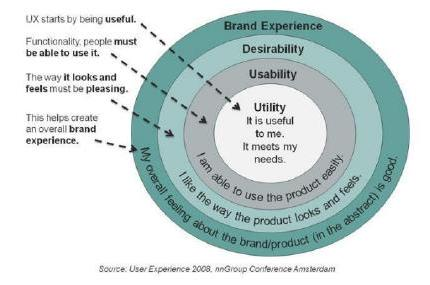
\includegraphics[width=0.6\linewidth]{images/2024_12_29_0d1d7b5551ea1b4b41bdg-02}
\end{concept}

\begin{definition}{Usability-Dimensionen nach ISO 9241}
\begin{itemize}
    \item \textbf{Effektivität:} Vollständige und genaue Zielerreichung
    \item \textbf{Effizienz:} Minimaler Aufwand für die Zielerreichung
    \item \textbf{Zufriedenheit:} Positive Nutzererfahrung
\end{itemize}
\end{definition}

\begin{theorem}{ISO 9241-110: Usability-Anforderungen}
\begin{itemize}
    \item \textbf{Aufgabenangemessenheit:} Unterstützung der Arbeitsaufgaben
    \item \textbf{Selbstbeschreibungsfähigkeit:} Verständliche Benutzerführung
    \item \textbf{Steuerbarkeit:} Kontrolle über Ablauf
    \item \textbf{Erwartungskonformität:} Konsistentes Verhalten
    \item \textbf{Fehlertoleranz:} Fehlervermeidung und -korrektur
    \item \textbf{Individualisierbarkeit:} Anpassung an Benutzergruppen
    \item \textbf{Lernförderlichkeit:} Unterstützung beim Lernen
\end{itemize}
\end{theorem}

\begin{KR}{Usability-Evaluation durchführen}
\begin{enumerate}
    \item \textbf{Vorbereitung}
    \begin{itemize}
        \item Testziele definieren
        \item Testpersonen auswählen
        \item Testaufgaben erstellen
    \end{itemize}
    \item \textbf{Durchführung}
    \begin{itemize}
        \item Beobachtung der Nutzer
        \item Protokollierung von Problemen
        \item Zeitmessung der Aufgaben
    \end{itemize}
    \item \textbf{Auswertung}
    \begin{itemize}
        \item Probleme klassifizieren
        \item Schweregrad bestimmen
        \item Verbesserungen vorschlagen
    \end{itemize}
\end{enumerate}
\end{KR}

\subsection{User-Centered Design (UCD)}

\begin{concept}{UCD Process}
Ein iterativer Prozess zur nutzerzentrierten Entwicklung:
\begin{itemize}
    \item User \& Domain Research
    \item Requirements Analysis  
    \item Design \& Prototype
    \item Evaluate
\end{itemize}
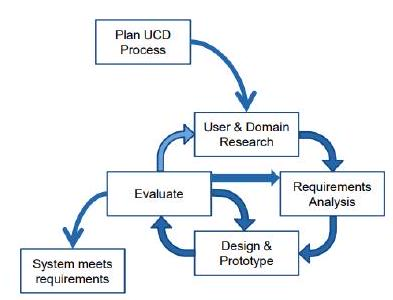
\includegraphics[width=0.9\linewidth]{images/2024_12_29_0d1d7b5551ea1b4b41bdg-03}
\end{concept}

\begin{KR}{User \& Domain Research}
\begin{enumerate}
    \item \textbf{Zielgruppe identifizieren}
    \begin{itemize}
        \item Wer sind die Benutzer?
        \item Aufgaben/Ziele verstehen 
        \item Arbeitsumgebung analysieren
    \end{itemize}
    \item \textbf{Daten sammeln}
    \begin{itemize}
        \item Contextual Inquiry
        \item Interviews/Beobachtungen
        \item Fokusgruppen
    \end{itemize}
    \item \textbf{Ergebnisse dokumentieren}
    \begin{itemize}
        \item Personas erstellen
        \item Usage-Szenarien beschreiben
        \item Mentales Modell entwickeln
    \end{itemize}
\end{enumerate}
\end{KR}

%todo: Add more examples for each artifact type (Personas, Usage-Scenarios, etc.)

\subsection{Requirements Engineering}

\begin{definition}{Requirements (Anforderungen)}
Kern-Eigenschaften von Anforderungen:
\begin{itemize}
    \item Explizit oder implizit
    \item Fast nie vollständig zu Beginn bekannt
    \item Mit allen Stakeholdern zu erarbeiten
    \item Entwickeln sich während des Projekts
    \item Müssen verifizierbar und messbar sein
\end{itemize}

\textbf{Herkunft:}
\begin{itemize}
    \item Benutzer (Ziele, Bedürfnisse, Kontext)  
    \item Weitere Stakeholder (Management, IT, etc.)
    \item Regulatorien, Gesetze, Normen
\end{itemize}

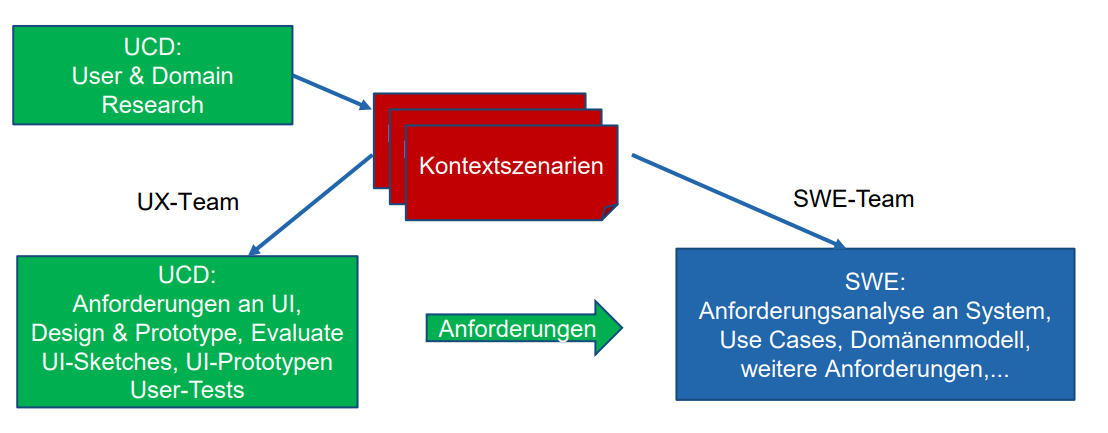
\includegraphics[width=\linewidth]{images/user_anforderungen.png}
\end{definition}

\begin{concept}{Arten von Anforderungen}
\textbf{Funktionale Anforderungen:}
\begin{itemize}
    \item Beschreiben, WAS das System tun soll
    \item Werden in Use Cases dokumentiert
    \item Müssen konkret und testbar sein
\end{itemize}

\textbf{Nicht-funktionale Anforderungen (ISO 25010):}
\begin{itemize}
    \item Performance Efficiency
    \item Compatibility 
    \item Usability
    \item Reliability
    \item Security
    \item Maintainability
    \item Portability
\end{itemize}

\textbf{Randbedingungen:}
\begin{itemize}
    \item Technische Einschränkungen
    \item Rechtliche Vorgaben
    \item Budgetäre Grenzen
    \item Zeitliche Limitationen
\end{itemize}
\end{concept}

\subsection{Use Cases}

\begin{definition}{Use Case (Anwendungsfall)}
Ein Use Case beschreibt eine konkrete Interaktion zwischen Akteur und System:

\textbf{Grundprinzipien:}
\begin{itemize}
    \item Aus Sicht des Akteurs beschrieben
    \item Aktiv formuliert (Verb + Objekt)
    \item Konkreter Nutzen für Akteur
    \item Mehr als eine einzelne Interaktion
    \item Essentieller Stil (Logik statt Implementierung)
\end{itemize}

\textbf{Qualitätskriterien:}
\begin{itemize}
    \item Boss-Test: Sinnvolle Arbeitseinheit
    \item EBP-Test: Elementary Business Process
    \item Size-Test: Mehrere Interaktionen
\end{itemize}
\end{definition}

\begin{concept}{Use Case Beziehungen}
\textbf{Include-Beziehung:}
\begin{itemize}
    \item Ein UC schließt einen anderen UC ein
    \item Wiederverwendung von Funktionalität
    \item Obligatorische Beziehung
\end{itemize}

\textbf{Extend-Beziehung:}
\begin{itemize}
    \item Optionale Erweiterung eines UC
    \item Unter bestimmten Bedingungen
    \item Ursprünglicher UC bleibt unverändert
\end{itemize}
\end{concept}

\begin{concept}{Use Case Granularität}
\begin{enumerate}
    \item \textbf{Brief Use Case}
    \begin{itemize}
        \item Kurze Zusammenfassung
        \item Hauptablauf skizzieren
        \item Keine Details zu Varianten
    \end{itemize}
    \item \textbf{Casual Use Case}
    \begin{itemize}
        \item Mehrere Absätze
        \item Hauptvarianten beschreiben
        \item Informeller Stil
    \end{itemize}
    \item \textbf{Fully-dressed Use Case}
    \begin{itemize}
        \item Vollständige Struktur
        \item Alle Varianten
        \item Vor- und Nachbedingungen
    \end{itemize}
\end{enumerate}
\end{concept}

\begin{KR}{Fully-dressed Use Case erstellen}
\begin{itemize}
    \item \textbf{Grundinformationen}
    \begin{itemize}
        \item Name (aktiv)
        \item Umfang (Scope)
        \item Ebene (Level)
        \item Primärakteur
    \end{itemize}
    \item \textbf{Stakeholder und Interessen}
    \begin{itemize}
        \item Alle beteiligten Parteien
        \item Deren spezifische Interessen
    \end{itemize}
    \item \textbf{Vor- und Nachbedingungen}
    \begin{itemize}
        \item Was muss vorher erfüllt sein?
        \item Was ist nachher garantiert?
    \end{itemize}
    \item \textbf{Standardablauf}
    \begin{itemize}
        \item Nummerierte Schritte
        \item Akteur-System-Interaktion
        \item Klare Erfolgskriterien
    \end{itemize}
    \item \textbf{Erweiterungen}
    \begin{itemize}
        \item Alternative Abläufe
        \item Fehlerszenarien
        \item Verzweigungen
    \end{itemize}
\end{itemize}
\end{KR}

%todo: Add example of each Use Case type (Brief, Casual, Fully-dressed)

\subsection{System Sequence Diagrams}

\begin{concept}{System Sequence Diagrams (SSD)}
\begin{itemize}
    \item Formalisierte Darstellung der System-Interaktionen
    \item Identifiziert Systemoperationen
    \item Basis für API-Design
    \item Abstrahiert von UI-Details
\end{itemize}
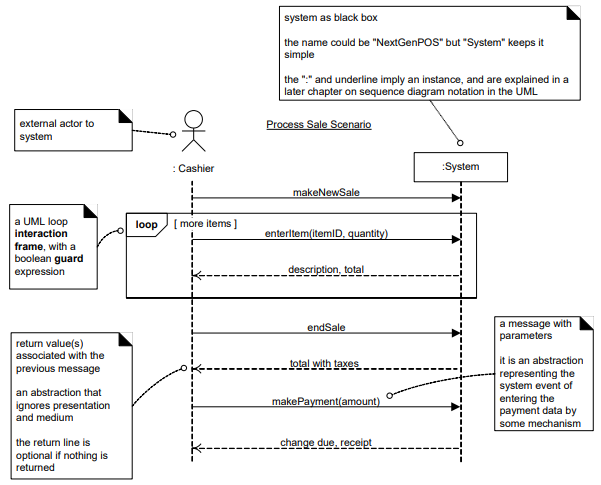
\includegraphics[width=\linewidth]{images/ssd.png}
\end{concept}

\begin{KR}{Contracts für Systemoperationen}
\textbf{1. Struktur}
\begin{itemize}
    \item Name und Parameter
    \item Querverweis zum Use Case
    \item Vorbedingungen
    \item Nachbedingungen
\end{itemize}

\textbf{2. Vorbedingungen}
\begin{itemize}
    \item Systemzustand vor Aufruf
    \item Notwendige Initialisierungen
    \item Gültige Parameter
\end{itemize}

\textbf{3. Nachbedingungen}
\begin{itemize}
    \item Erstellte/gelöschte Instanzen
    \item Geänderte Attribute
    \item Neue/gelöschte Assoziationen
\end{itemize}
\end{KR}

%todo: Add SSD examples and Operation Contract examples